\documentclass[ngerman, 11pt, a4paper]{article}

\usepackage[left=2cm, right=2cm, top=2cm, bottom=2cm]{geometry}
\usepackage{fontspec}
\usepackage{parskip}
\usepackage{caption}
\captionsetup[listing]{position=top}
\usepackage{booktabs}
\usepackage{graphicx}
\usepackage[hidelinks]{hyperref}
\usepackage[hang,multiple,bottom]{footmisc} 
\usepackage{enumitem}
\usepackage{tablefootnote}
\usepackage{float}
\usepackage{etoolbox}
\usepackage[ngerman]{babel}
\usepackage{sectsty}
\usepackage[nottoc]{tocbibind}

\usepackage{xltxtra} 
\defaultfontfeatures{Mapping=tex-text} 

\usepackage{polyglossia} 
\setdefaultlanguage[spelling=new]{german} 

\AfterEndEnvironment{figure}{\vspace{-15pt}}
\AfterEndEnvironment{table}{\vspace{-15pt}}

\setitemize{noitemsep}

\usepackage[
  backend=biber
 ,style=apa
 ,sortlocale=de_DE 
 ,sorting=nyvt
 ,sortcites=false
 ,block=none
 ,url=true
 ,urldate=comp
 ,minnames=1
 ,maxnames=3
]{biblatex}
\addbibresource{bibliography.bib}
\DeclareLanguageMapping{german}{german-apa} 

\DefineBibliographyStrings{ngerman}{
  urlfrom   = {verfügbar unter},
  retrieved = {letzter Zugriff am},
  from      = {von:}
}

\sectionfont{\fontsize{12}{12}\selectfont}
\subsectionfont{\fontsize{12}{12}\selectfont}
\subsubsectionfont{\fontsize{12}{12}\selectfont}
\renewcommand{\footnotesize}{\linespread{1}\fontsize{10pt}{12pt}\selectfont}

\setmainfont{Arial}
\linespread{1.5}

\newlist{abbrv}{itemize}{1}
\setlist[abbrv,1]{label=,labelwidth=1in,align=parleft,itemsep=0.1\baselineskip,leftmargin=!}

% https://tex.stackexchange.com/a/246285
\graphicspath{{images/}}

\renewcommand{\footnotesize}{\linespread{1}\fontsize{10pt}{12pt}\selectfont}
\newcommand{\source}[1]{\caption*{\footnotesize Quelle: {#1}} }
\newcommand{\tablesource}[1]{\vspace{10pt} \caption*{\footnotesize Quelle: {#1}} }

\begin{document}

\pagenumbering{Roman}

\section*{Abstract}
\addcontentsline{toc}{section}{Abstract}

Lorem ipsum dolor sit amet, consectetuer adipiscing elit. Aenean commodo ligula eget dolor. Aenean massa. Cum sociis natoque penatibus et magnis dis parturient montes, nascetur ridiculus mus. Donec quam felis, ultricies nec, pellentesque eu, pretium quis, sem. Nulla consequat massa quis enim. Donec pede justo, fringilla vel, aliquet nec, vulputate eget, arcu.

In enim justo, rhoncus ut, imperdiet a, venenatis vitae, justo. Nullam dictum felis eu pede mollis pretium. Integer tincidunt. Cras dapibus. Vivamus elementum semper nisi. Aenean vulputate eleifend tellus. Aenean leo ligula, porttitor eu, consequat vitae, eleifend ac, enim. Aliquam lorem ante, dapibus in, viverra quis, feugiat a, tellus.

Phasellus viverra nulla ut metus varius laoreet. Quisque rutrum. Aenean imperdiet. Etiam ultricies nisi vel augue. Curabitur ullamcorper ultricies nisi. Nam eget dui. Etiam rhoncus. Maecenas tempus, tellus eget condimentum rhoncus, sem quam semper libero, sit amet adipiscing sem neque sed ipsum. Nam quam nunc, blandit vel, luctus pulvinar, hendrerit id, lorem.

Maecenas nec odio et ante tincidunt tempus. Donec vitae sapien ut libero venenatis faucibus. Nullam quis ante. Etiam sit amet orci eget eros faucibus tincidunt. Duis leo. Sed fringilla mauris sit amet nibh. Donec sodales sagittis magna. Sed consequat, leo eget bibendum sodales, augue velit cursus nunc, quis gravida magna mi a libero. Fusce vulputate eleifend sapien.

\pagebreak
\renewcommand{\contentsname}{Inhaltsverzeichnis}
\tableofcontents
\pagebreak

\listoffigures
\pagebreak

\section*{Abkürzungsverzeichnis}
\addcontentsline{toc}{section}{Abkürzungsverzeichnis}

\begin{abbrv}

\item[ABC] Lorem ipsum dolor sit amet
\item[XYZ] Maecenas nec odio et ante tincidunt tempus
 
\end{abbrv}
\pagebreak

\pagenumbering{arabic}

\section{Trapattoni '98}

\subsection{Die Rede}

Es gibt im Moment in diese Mannschaft\footnote{Gemeint ist die Mannschaft des FC Bayern München in der Saison 1997/98.}, oh, einige Spieler vergessen ihnen Profi was sie sind. Ich lese nicht sehr viele Zeitungen, aber ich habe gehört viele Situationen. Erstens: wir haben nicht offensiv gespielt. Es gibt keine deutsche Mannschaft spielt offensiv und die Name offensiv wie Bayern.

Letzte Spiel hatten wir in Platz drei Spitzen: Elber, Jancka und dann Zickler. Wir müssen nicht vergessen Zickler. Zickler ist eine Spitzen mehr, Mehmet eh mehr Basler. Ist klar diese Wörter, ist möglich verstehen, was ich hab gesagt? Danke. Offensiv, offensiv ist wie machen wir in Platz.

\subsection{Zweitens}

 Zweitens: ich habe erklärt mit diese zwei Spieler: nach Dortmund brauchen vielleicht Halbzeit Pause. Ich habe auch andere Mannschaften gesehen in Europa nach diese Mittwoch. Ich habe gesehen auch zwei Tage die Training. Ein Trainer ist nicht ein Idiot! Ein Trainer sei sehen was passieren in Platz.
 
\subsection{Leere Flasche}

 In diese Spiel es waren zwei, drei diese Spieler waren schwach wie eine Flasche leer! Haben Sie gesehen Mittwoch, welche Mannschaft hat gespielt Mittwoch? Hat gespielt Mehmet oder gespielt Basler oder hat gespielt Trapattoni? Diese Spieler beklagen mehr als sie spielen! Wissen Sie, warum die Italienmannschaften kaufen nicht diese Spieler? Weil wir haben gesehen viele Male solche Spiel!
 
 \subsubsection{Was erlauben Strunz}
 
  Hat gespielt Mehmet oder gespielt Basler oder hat gespielt Trapattoni? Diese Spieler beklagen mehr als sie spielen! Wissen Sie, warum die Italienmannschaften kaufen nicht diese Spieler? Weil wir haben gesehen viele Male solche Spiel! Haben gesagt sind nicht Spieler für die italienisch Meisters! Strunz! Strunz ist zwei Jahre hier, hat gespielt 10 Spiele, ist immer verletzt! Was erlauben Strunz? Letzte Jahre Meister Geworden mit Hamann, eh, Nerlinger. Diese Spieler waren Spieler! Waren Meister geworden! Ist immer verletzt!
  
  \subsubsection{25 Spiele!}
  
   Hat gespielt 25 Spiele in diese Mannschaft in diese Verein. Muß respektieren die andere Kollegen! haben viel nette kollegen! Stellen Sie die Kollegen die Frage! Haben keine Mut an Worten, aber ich weiß, was denken über diese Spieler. Mussen zeigen jetzt, ich will, Samstag, diese Spieler müssen zeigen mich, seine Fans, müssen alleine die Spiel gewinnen. Muß allein die Spiel gewinnen!
   
\section{Kafka}

\subsection{Verleumdung}

Jemand musste Josef K. verleumdet haben, denn ohne dass er etwas Böses getan hätte, wurde er eines Morgens verhaftet \parencite{mitrednf2021}. »Wie ein Hund! « sagte er, es war, als sollte die Scham ihn überleben. Als Gregor Samsa eines Morgens aus unruhigen Träumen erwachte, fand er sich in seinem Bett zu einem ungeheueren Ungeziefer verwandelt. Und es war ihnen wie eine Bestätigung ihrer neuen Träume und guten Absichten, als am Ziele ihrer Fahrt die Tochter als erste sich erhob und ihren jungen Körper dehnte.

\subsection{Eigentümlicher Apparat}

 »Es ist ein eigentümlicher Apparat«, sagte der Offizier zu dem Forschungsreisenden und überblickte mit einem gewissermaßen bewundernden Blick den ihm doch wohlbekannten Apparat \parencite{syme2011f}. Sie hätten noch ins Boot springen können, aber der Reisende hob ein schweres, geknotetes Tau vom Boden, drohte ihnen damit und hielt sie dadurch von dem Sprunge ab. In den letzten Jahrzehnten ist das Interesse an Hungerkünstlern sehr zurückgegangen. Aber sie überwanden sich, umdrängten den Käfig und wollten sich gar nicht fortrühren. 
 
\begin{figure}[H]
\centering
\caption{Die Bezeichnung einer eingebetteten Grafik}
\label{fig:chasm}
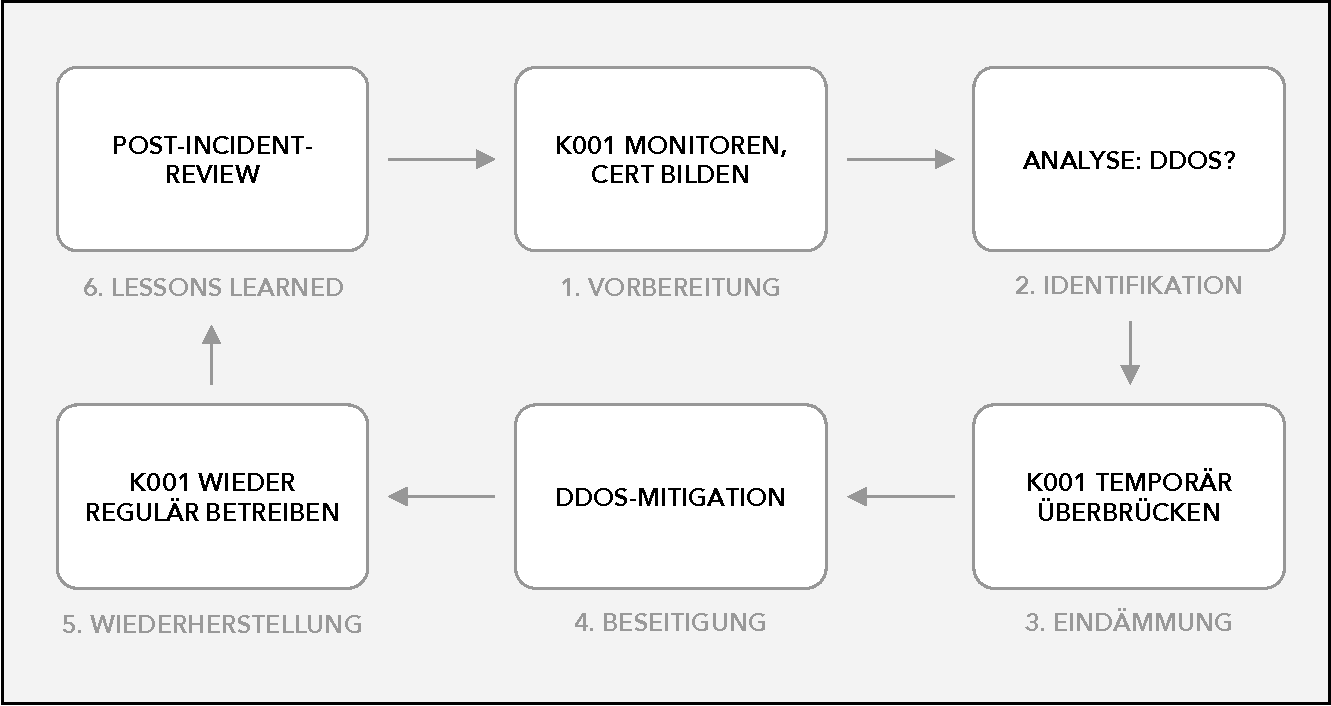
\includegraphics[width=\textwidth]{graphic}
\source{Eigene Darstellung}
\end{figure} 

\section{Fazit}

Überall dieselbe alte Leier. Das Layout ist fertig, der Text lässt auf sich warten. Damit das Layout nun nicht nackt im Raume steht und sich klein und leer vorkommt, springe ich ein: der Blindtext. Genau zu diesem Zwecke erschaffen, immer im Schatten meines großen Bruders »Lorem Ipsum«, freue ich mich jedes Mal, wenn Sie ein paar Zeilen lesen. Denn esse est percipi - Sein ist wahrgenommen werden.

Und weil Sie nun schon die Güte haben, mich ein paar weitere Sätze lang zu begleiten, möchte ich diese Gelegenheit nutzen, Ihnen nicht nur als Lückenfüller zu dienen, sondern auf etwas hinzuweisen, das es ebenso verdient wahrgenommen zu werden: Webstandards nämlich. Sehen Sie, Webstandards sind das Regelwerk, auf dem Webseiten aufbauen. So gibt es Regeln für HTML, CSS, JavaScript oder auch XML; Worte, die Sie vielleicht schon einmal von Ihrem Entwickler gehört haben. Diese Standards sorgen dafür, dass alle Beteiligten aus einer Webseite den größten Nutzen ziehen.

Im Gegensatz zu früheren Webseiten müssen wir zum Beispiel nicht mehr zwei verschiedene Webseiten für den Internet Explorer und einen anderen Browser programmieren. Es reicht eine Seite, die - richtig angelegt - sowohl auf verschiedenen Browsern im Netz funktioniert, aber ebenso gut für den Ausdruck oder die Darstellung auf einem Handy geeignet ist. Wohlgemerkt: Eine Seite für alle Formate. Was für eine Erleichterung. Standards sparen Zeit bei den Entwicklungskosten und sorgen dafür, dass sich Webseiten später leichter pflegen lassen. Natürlich nur dann, wenn sich alle an diese Standards halten.

Das gilt für Browser wie Firefox, Opera, Safari und den Internet Explorer ebenso wie für die Darstellung in Handys. Und was können Sie für Standards tun? Fordern Sie von Ihren Designern und Programmieren einfach standardkonforme Webseiten. Ihr Budget wird es Ihnen auf Dauer danken. Ebenso möchte ich Ihnen dafür danken, dass Sie mich bis zum Ende gelesen haben. Meine Mission ist erfüllt. Ich werde hier noch die Stellung halten, bis der geplante Text eintrifft. Ich wünsche Ihnen noch einen schönen Tag. Und arbeiten Sie nicht zuviel! Überall dieselbe alte Leier.

\pagebreak
\pagenumbering{Roman}
\setcounter{page}{3}

\setcounter{biburllcpenalty}{7000}
\setcounter{biburlucpenalty}{8000}

\printbibliography[title=Literaturverzeichnis, heading=bibintoc]

\end{document}

